\documentclass{standalone}
\usepackage{tikz}
\usetikzlibrary{patterns, positioning}
\usepackage[sfdefault]{ClearSans} %% option 'sfdefault' activates Clear Sans as the default text font
\usepackage[T1]{fontenc}

\begin{document}
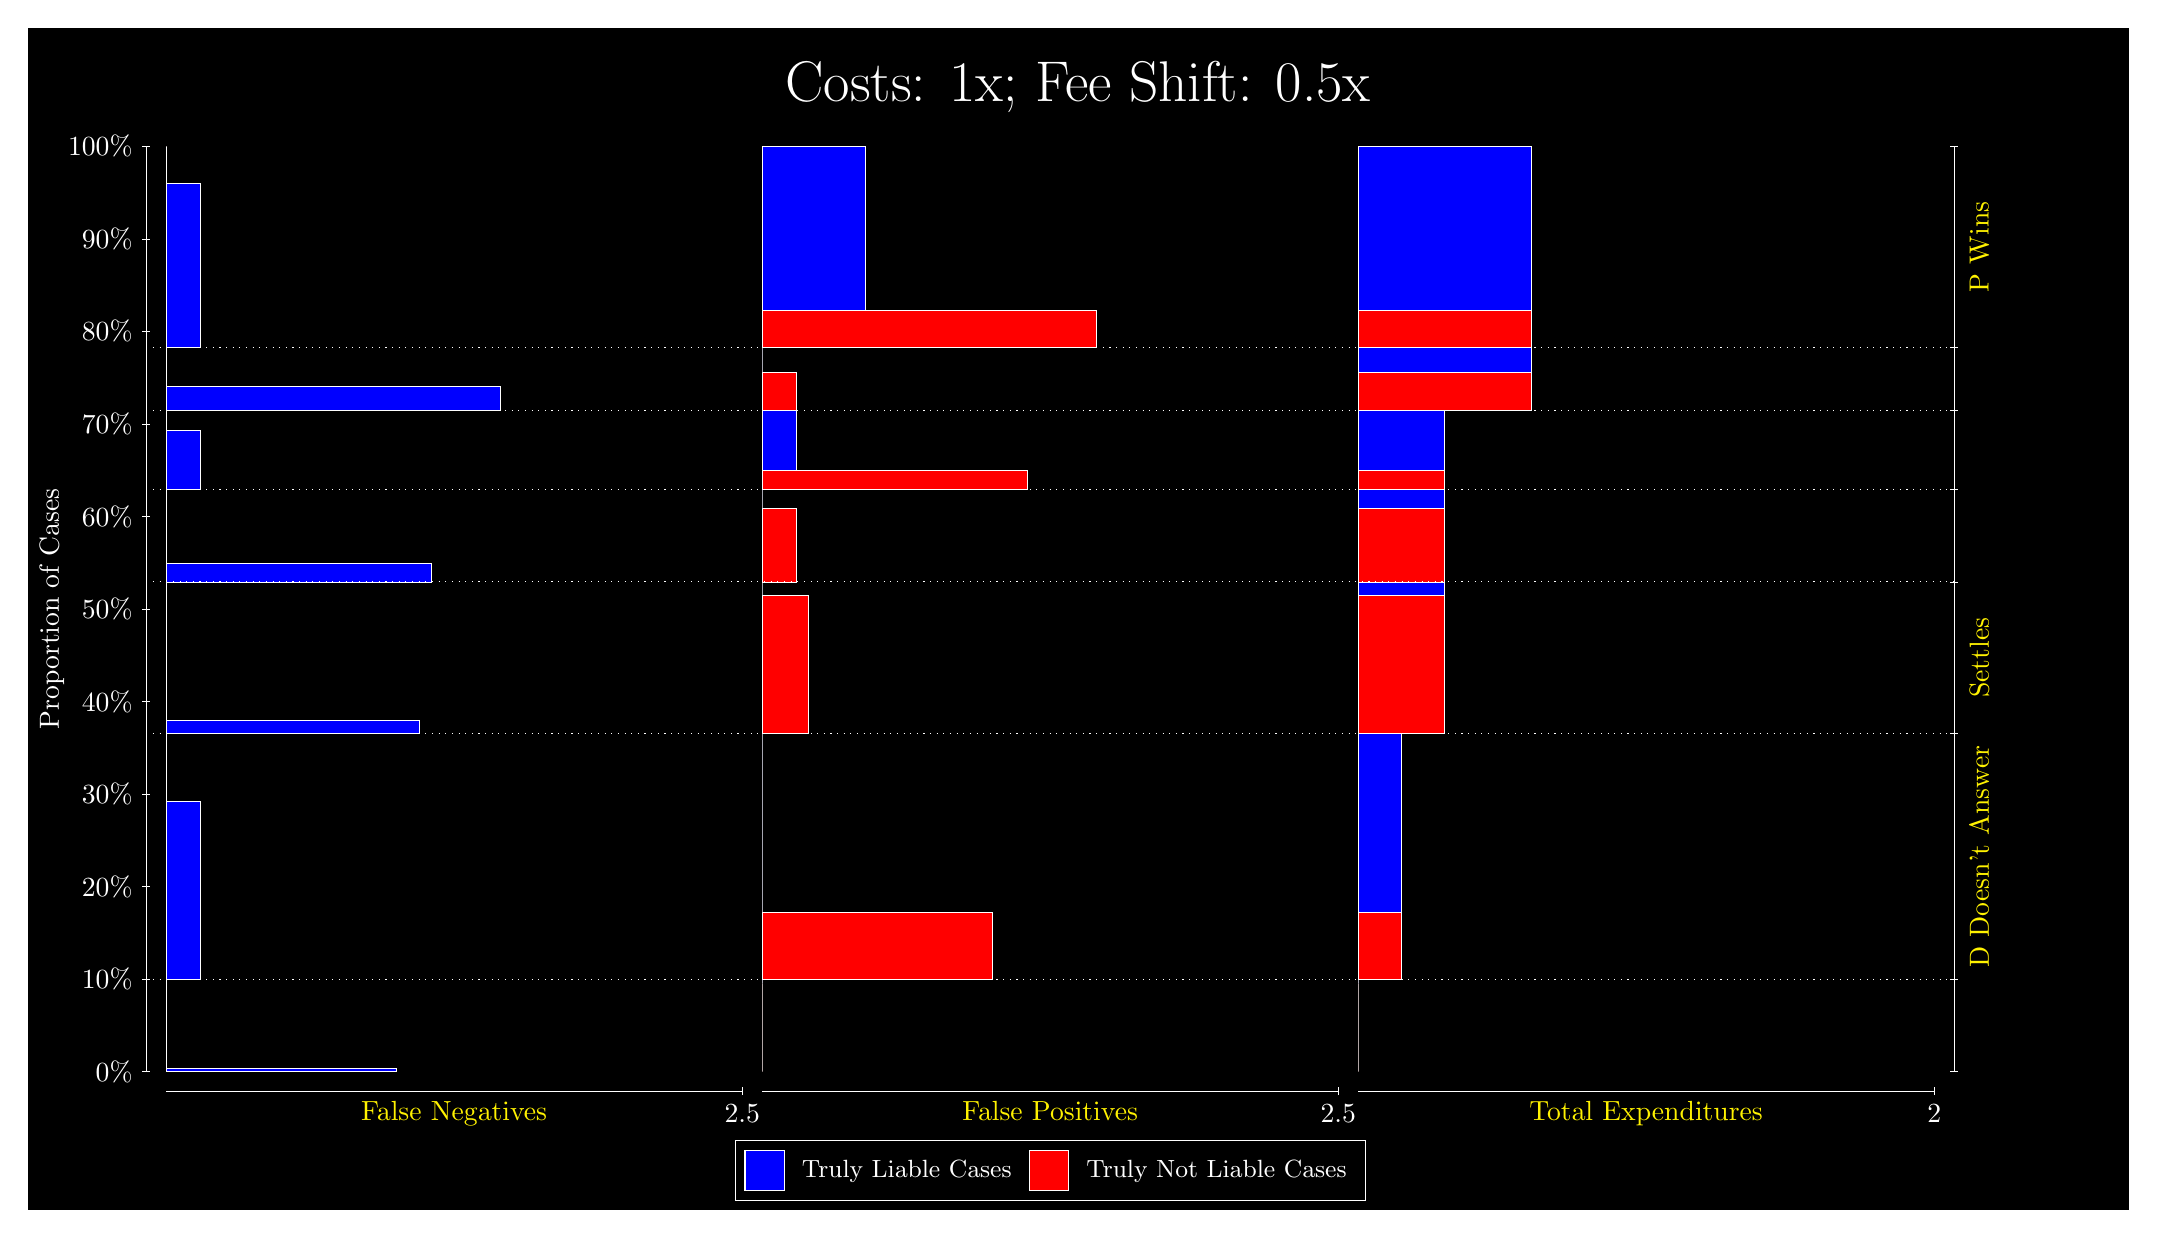
\begin{tikzpicture}
\draw[fill=black] (0,0) rectangle (26.667,15);
\draw[text=white] (0,13.5) rectangle (26.667,15) node[midway] {\huge Costs: 1x; Fee Shift: 0.5x};
\draw[white, very thin] (1.5,1.75) -- (1.5,13.5);
\node[rotate=90, text=white, anchor=center] at (0.3, 7.625) {Proportion of Cases};
\draw[white, very thin] (1.45,1.75) -- (1.55,1.75);
\node[text=white, anchor=east] at (1.45, 1.75) {0\%};
\draw[white, very thin] (1.45,2.925) -- (1.55,2.925);
\node[text=white, anchor=east] at (1.45, 2.925) {10\%};
\draw[white, very thin] (1.45,4.1) -- (1.55,4.1);
\node[text=white, anchor=east] at (1.45, 4.1) {20\%};
\draw[white, very thin] (1.45,5.275) -- (1.55,5.275);
\node[text=white, anchor=east] at (1.45, 5.275) {30\%};
\draw[white, very thin] (1.45,6.45) -- (1.55,6.45);
\node[text=white, anchor=east] at (1.45, 6.45) {40\%};
\draw[white, very thin] (1.45,7.625) -- (1.55,7.625);
\node[text=white, anchor=east] at (1.45, 7.625) {50\%};
\draw[white, very thin] (1.45,8.8) -- (1.55,8.8);
\node[text=white, anchor=east] at (1.45, 8.8) {60\%};
\draw[white, very thin] (1.45,9.975) -- (1.55,9.975);
\node[text=white, anchor=east] at (1.45, 9.975) {70\%};
\draw[white, very thin] (1.45,11.15) -- (1.55,11.15);
\node[text=white, anchor=east] at (1.45, 11.15) {80\%};
\draw[white, very thin] (1.45,12.325) -- (1.55,12.325);
\node[text=white, anchor=east] at (1.45, 12.325) {90\%};
\draw[white, very thin] (1.45,13.5) -- (1.55,13.5);
\node[text=white, anchor=east] at (1.45, 13.5) {100\%};

\draw[white, very thin] (24.457,1.75) -- (24.457,13.5);
\draw[white, very thin] (24.407,1.75) -- (24.507,1.75);
\node[anchor=west] at (24.407, 1.75) {};
\draw[white, very thin] (24.407,2.9178) -- (24.507,2.9178);
\node[anchor=west] at (24.407, 2.9178) {};
\draw[white, very thin] (24.407,6.0407) -- (24.507,6.0407);
\node[anchor=west] at (24.407, 6.0407) {};
\draw[white, very thin] (24.407,7.9686) -- (24.507,7.9686);
\node[anchor=west] at (24.407, 7.9686) {};
\draw[white, very thin] (24.407,9.1411) -- (24.507,9.1411);
\node[anchor=west] at (24.407, 9.1411) {};
\draw[white, very thin] (24.407,10.142) -- (24.507,10.142);
\node[anchor=west] at (24.407, 10.142) {};
\draw[white, very thin] (24.407,10.946) -- (24.507,10.946);
\node[anchor=west] at (24.407, 10.946) {};
\draw[white, very thin] (24.407,13.5) -- (24.507,13.5);
\node[anchor=west] at (24.407, 13.5) {};

\draw[white, very thin, fill=blue] (1.75,1.75) rectangle (4.6775,1.7976);
\draw[white, very thin, fill=red] (1.75,1.7976) rectangle (1.75,2.9178);
\draw[white, very thin, fill=blue] (1.75,2.9178) rectangle (2.1891,5.183);
\draw[white, very thin, fill=red] (1.75,5.183) rectangle (1.75,6.0407);
\draw[white, very thin, fill=blue] (1.75,6.0407) rectangle (4.9703,6.2104);
\draw[white, very thin, fill=red] (1.75,6.2104) rectangle (1.75,7.9686);
\draw[white, very thin, fill=blue] (1.75,7.9686) rectangle (5.1167,8.2072);
\draw[white, very thin, fill=red] (1.75,8.2072) rectangle (1.75,9.1411);
\draw[white, very thin, fill=blue] (1.75,9.1411) rectangle (2.1891,9.8938);
\draw[white, very thin, fill=red] (1.75,9.8938) rectangle (1.75,10.142);
\draw[white, very thin, fill=blue] (1.75,10.142) rectangle (5.9949,10.455);
\draw[white, very thin, fill=red] (1.75,10.455) rectangle (1.75,10.946);
\draw[white, very thin, fill=blue] (1.75,10.946) rectangle (2.1891,13.034);
\draw[white, very thin, fill=red] (1.75,13.034) rectangle (1.75,13.5);
\draw[white, very thin, fill=red] (9.3189,1.75) rectangle (9.3189,2.8703);
\draw[white, very thin, fill=blue] (9.3189,2.8703) rectangle (9.3189,2.9178);
\draw[white, very thin, fill=red] (9.3189,2.9178) rectangle (12.246,3.7756);
\draw[white, very thin, fill=blue] (9.3189,3.7756) rectangle (9.3189,6.0407);
\draw[white, very thin, fill=red] (9.3189,6.0407) rectangle (9.9044,7.799);
\draw[white, very thin, fill=blue] (9.3189,7.799) rectangle (9.3189,7.9686);
\draw[white, very thin, fill=red] (9.3189,7.9686) rectangle (9.758,8.9025);
\draw[white, very thin, fill=blue] (9.3189,8.9025) rectangle (9.3189,9.1411);
\draw[white, very thin, fill=red] (9.3189,9.1411) rectangle (12.686,9.3895);
\draw[white, very thin, fill=blue] (9.3189,9.3895) rectangle (9.758,10.142);
\draw[white, very thin, fill=red] (9.3189,10.142) rectangle (9.758,10.633);
\draw[white, very thin, fill=blue] (9.3189,10.633) rectangle (9.3189,10.946);
\draw[white, very thin, fill=red] (9.3189,10.946) rectangle (13.564,11.412);
\draw[white, very thin, fill=blue] (9.3189,11.412) rectangle (10.636,13.5);
\draw[white, very thin, fill=red] (16.888,1.75) rectangle (16.888,2.8703);
\draw[white, very thin, fill=blue] (16.888,2.8703) rectangle (16.888,2.9178);
\draw[white, very thin, fill=red] (16.888,2.9178) rectangle (17.437,3.7756);
\draw[white, very thin, fill=blue] (16.888,3.7756) rectangle (17.437,6.0407);
\draw[white, very thin, fill=red] (16.888,6.0407) rectangle (17.986,7.799);
\draw[white, very thin, fill=blue] (16.888,7.799) rectangle (17.986,7.9686);
\draw[white, very thin, fill=red] (16.888,7.9686) rectangle (17.986,8.9025);
\draw[white, very thin, fill=blue] (16.888,8.9025) rectangle (17.986,9.1411);
\draw[white, very thin, fill=red] (16.888,9.1411) rectangle (17.986,9.3895);
\draw[white, very thin, fill=blue] (16.888,9.3895) rectangle (17.986,10.142);
\draw[white, very thin, fill=red] (16.888,10.142) rectangle (19.083,10.633);
\draw[white, very thin, fill=blue] (16.888,10.633) rectangle (19.083,10.946);
\draw[white, very thin, fill=red] (16.888,10.946) rectangle (19.083,11.412);
\draw[white, very thin, fill=blue] (16.888,11.412) rectangle (19.083,13.5);
\draw[white, dotted] (1.5,2.9178) -- (24.457,2.9178);
\draw[white, dotted] (1.5,6.0407) -- (24.457,6.0407);
\draw[white, dotted] (1.5,7.9686) -- (24.457,7.9686);
\draw[white, dotted] (1.5,9.1411) -- (24.457,9.1411);
\draw[white, dotted] (1.5,10.142) -- (24.457,10.142);
\draw[white, dotted] (1.5,10.946) -- (24.457,10.946);
\draw[white, very thin] (1.75,1.5) -- (9.0689,1.5);
\node[text=yellow, anchor=north] at (5.4094, 1.5) {False Negatives};
\draw[white, very thin] (9.0689,1.45) -- (9.0689,1.55);
\node[text=white, anchor=north] at (9.0689, 1.45) {2.5};

\draw[white, very thin] (9.3189,1.5) -- (16.638,1.5);
\node[text=yellow, anchor=north] at (12.978, 1.5) {False Positives};
\draw[white, very thin] (16.638,1.45) -- (16.638,1.55);
\node[text=white, anchor=north] at (16.638, 1.45) {2.5};

\draw[white, very thin] (16.888,1.5) -- (24.207,1.5);
\node[text=yellow, anchor=north] at (20.547, 1.5) {Total Expenditures};
\draw[white, very thin] (24.207,1.45) -- (24.207,1.55);
\node[text=white, anchor=north] at (24.207, 1.45) {2};


\node[text=yellow, centered, rotate=90] at (24.777, 4.4793) {D Doesn't Answer};
\node[text=yellow, centered, rotate=90] at (24.777, 7.0047) {Settles};



\node[text=yellow, centered, rotate=90] at (24.777, 12.223) {P Wins};

\draw (12.978300999999998,1.5) node[draw=none] (baseCoordinate) {};
\begin{scope}[align=center]
        \matrix[scale=0.5, draw=white, below=0.5cm of baseCoordinate, nodes={draw}, column sep=0.1cm]{
            \node[rectangle, draw, minimum width=0.5cm, minimum height=0.5cm, fill=blue] {}; &
            \node[draw=none, font=\small, text=white] (B) {Truly Liable Cases}; &
            \node[rectangle, draw, minimum width=0.5cm, minimum height=0.5cm, fill=red] {}; &
            \node[draw=none, font=\small, text=white] (B) {Truly Not Liable Cases}; \\
            };
\end{scope}

\end{tikzpicture}
\end{document}